
\section{Scheduler}

	\begin{frame}{Master-Worker}
		\centerline{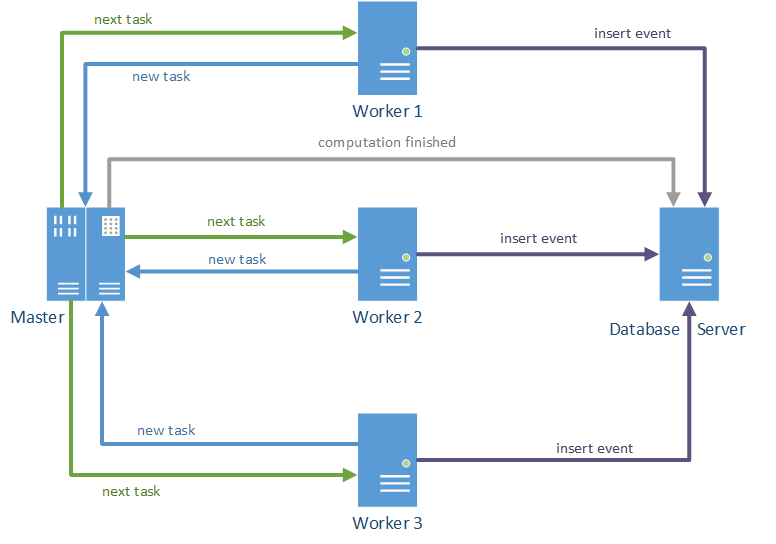
\includegraphics[scale=0.5]{images/master}}
	\end{frame}
	\begin{frame}{Task Stealing}
		\centerline{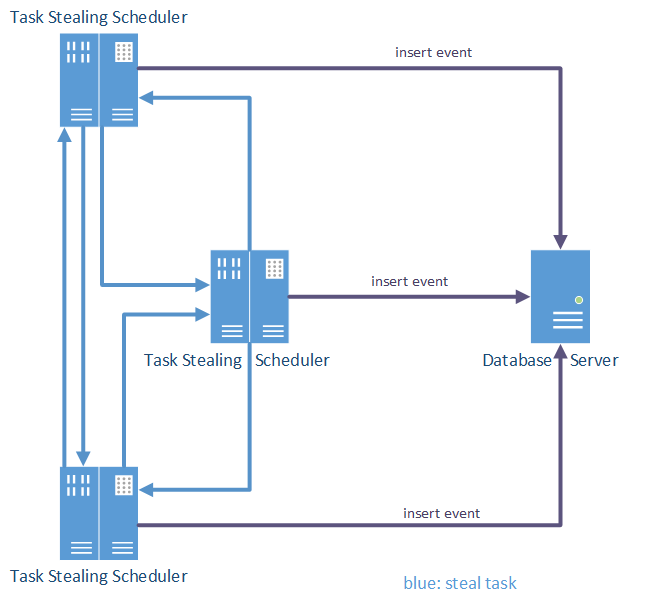
\includegraphics[scale=0.5]{images/taskstealing}}
	\end{frame}

	\begin{frame}{Scheduling strategies}
	\begin{minipage}[]{.7\textwidth}%
			\begin{itemize}
		\item<1-> non-statistical
		\begin{itemize}
			\item First In-First out (FIFO)
			\item Last In-Last out (LIFO)
		\end{itemize}
		\item<2-> statistical
		\begin{itemize}
			\item Shortest job first (SJF)
			\item Longest job first (LJF)
		\end{itemize}
		\item<3-> standardized interface - simple to include new strategies
		\end{itemize}
\end{minipage}%
\begin{minipage}[]{.3\textwidth}%
  \vspace{-\ht\strutbox}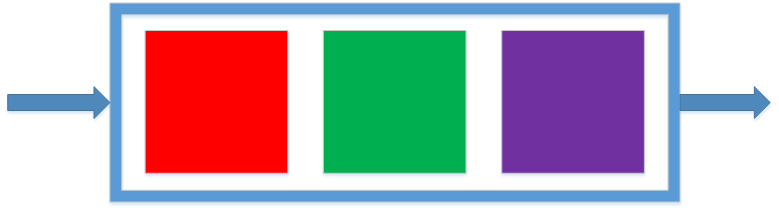
\includegraphics[width=\textwidth]{images/fifo}%
\end{minipage}		
		
	\end{frame}
	\begin{frame}{Scheduling strategies: Master-Worker vs. Task stealing}
		\begin{itemize}
			\item<1-> Master-Worker
				\begin{itemize}
					\item fast standard c++ implementation
					\item dynamic size
					\item easy to switch between scheduling strategies at runtime	
				\end{itemize}
			
			\item<2-> Task stealing
					\begin{itemize}
						\item custom implementation inside a MPI-Window
					\end{itemize}
			
		\end{itemize}
	\end{frame}